\chapter{Fairness Constraint Timing}
\todo{Need specifically mention these are tests for FAIRRET more across this whole chapter}
The point during training at which a fairness constraint should be introduced is not necessarily clear. Applying a fairness constraint for a longer portion of training gives the constraint more opportunity to influence the model, but may also limit the model's ability to optimise its predictive performance. Conversely, introducing the constraint later in training may allow the model to first focus on predictive performance before adjusting its behaviour to satisfy the fairness requirement. It is therefore unclear whether fairness constraints should influence the model throughout training or whether applying them only during later stages can achieve a better trade-off between fairness and predictive performance.

A later application of fairness constraints would be desirable if it can achieve comparable fairness to applying the constraint throughout training. This would allow the constraint strengths to be adjusted during the later stages of training to target specific fairness or performance requirements without having to retrain the model fully. Furthermore, if the effect of the constraint is largely determined during the final stages of training, only a partially trained model would be required when evaluating different constraint configurations. This could substantially reduce the computational cost of finding a suitable constraint strength and training configuration.

This experiment therefore investigates whether fairness constraints can be introduced later during training while still achieving comparable fairness and predictive performance to models constrained throughout training.

\section{Methodology}
The effect of the timing of fairness constraint application is evaluated by comparing models that are trained with varying lenths of fairness-constrained training. The experiment is performed on the ACSIncome, ACSEmployment and Law School datasets for each of the seven fairness metrics considered in this work.

For each dataset and fairness metric, a baseline model is first trained without a fairness constraint. A fully constrained model is trained separately using the same training configuration, with the fairness constraint applied throughout the entire training process. Additional models are created by branching from the baseline model at different intervals during training. From the point at which a model is branched, the corresponding fairness constraint is applied for the remainder of training. This results in models that spend different proportions of their training under the fairness constraint.

The resulting models are evaluated using predictive performance and fairness violation. Performance is plotted against fairness violation for the different constraint starting points, allowing the trade-off between the two measures to be compared. The fully constrained and unconstrained models are included as reference points.

\section{Results}
\subsection{Overall performance}
The effect of fairness constraint timing across the seven fairness metrics is shown in Figures \ref{fig:timingDP} to \ref{fig:timingTE}. Each figure compares the predictive performance and fairness violation resulting from introducing the constraint at different points during training.

Across nearly all evaluated configurations, a consistent pattern can be observed in which predictive performance decreases as the model is trained with the fairness constraint for a longer period. In most cases, this decrease in performance is not accompanied by a substantial improvement in the corresponding fairness violation. For some metrics, extending the duration of constrained training produces almost no or nearly no additional improvement in violation.

ACC \ref{fig:timingACC} provides an example where longer constrained training continues to improve the fairness violation, whereas DP \ref{fig:timingDP} shows a case where the violation changes little despite the additional constrained training. This indicates that the benefit of applying a fairness constraint for a longer period depends on the specific fairness metric.

Some results for the Law School dataset show substantially greater instability, particularly for PE and TE. These results make the effect of constraint timing less clear and are therefore less suitable for drawing conclusions about the general relationship between constraint duration, fairness, and predictive performance.

\begin{figure}[htbp]
    \centering
    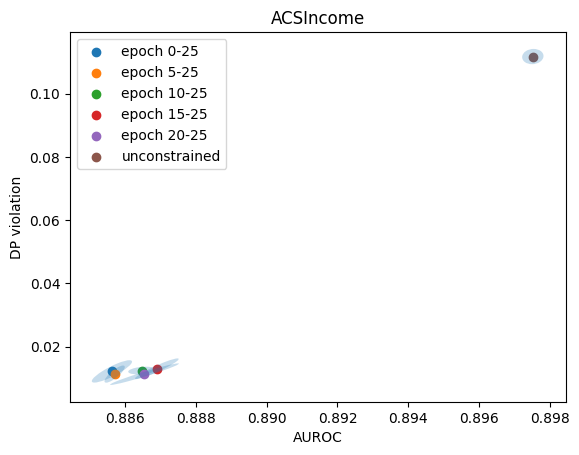
\includegraphics[width=0.45\textwidth]{assets/timing/ACSIncome-DP.png}
    \hfill
    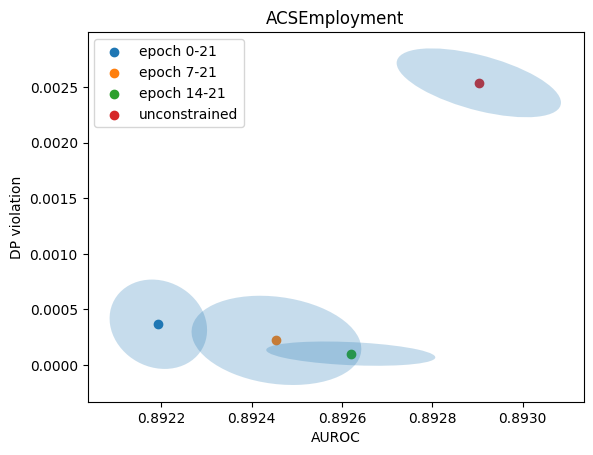
\includegraphics[width=0.45\textwidth]{assets/timing/ACSEmployment-DP.png}
    \hfill
    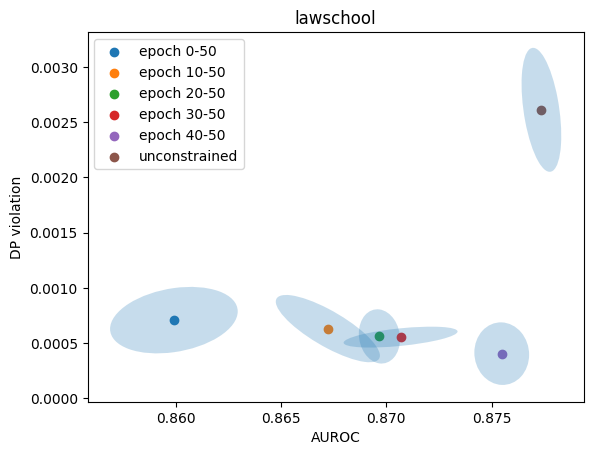
\includegraphics[width=0.45\textwidth]{assets/timing/lawschool-DP.png}
    \caption{DP perfomance plots using different ranges of fairness constrained training.}
    \label{fig:timingDP}
\end{figure}
    
\begin{figure}[htbp]
    \centering
    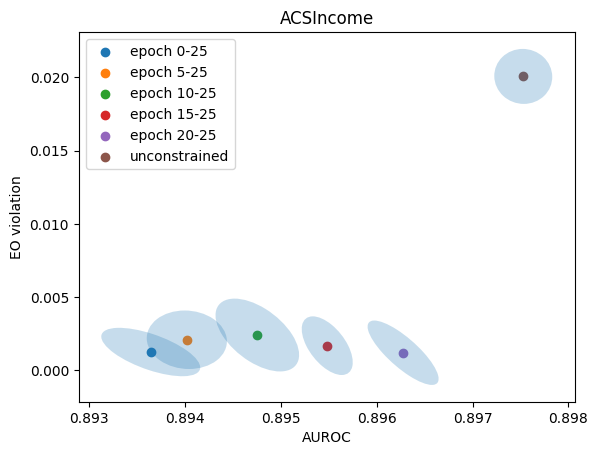
\includegraphics[width=0.45\textwidth]{assets/timing/ACSIncome-EO.png}
    \hfill
    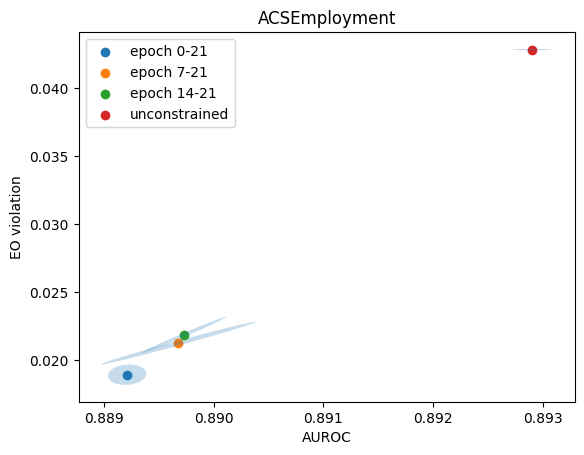
\includegraphics[width=0.45\textwidth]{assets/timing/ACSEmployment-EO.png}
    \hfill
    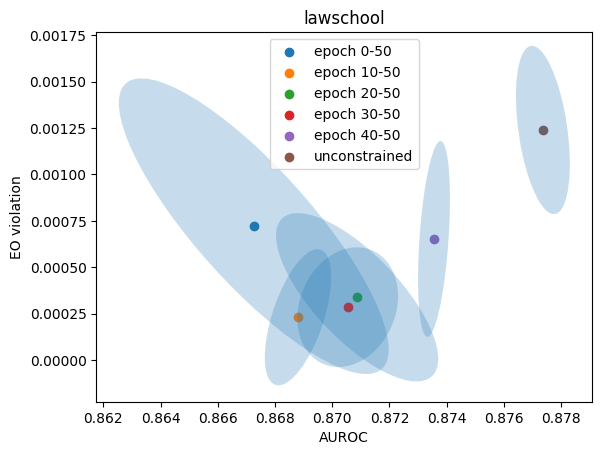
\includegraphics[width=0.45\textwidth]{assets/timing/lawschool-EO.png}
    \caption{EO perfomance plots using different ranges of fairness constrained training.}
\end{figure}
    
\begin{figure}[htbp]
    \centering
    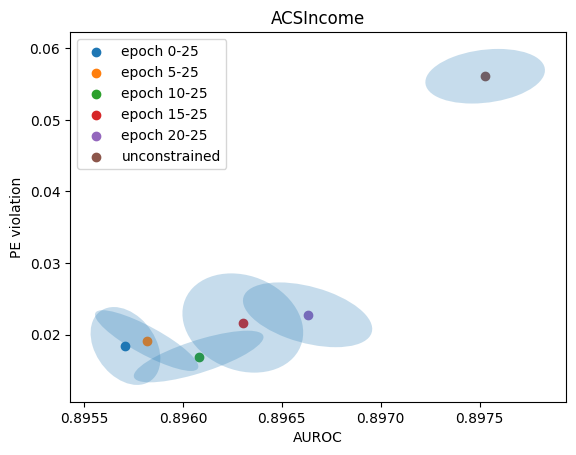
\includegraphics[width=0.45\textwidth]{assets/timing/ACSIncome-PE.png}
    \hfill
    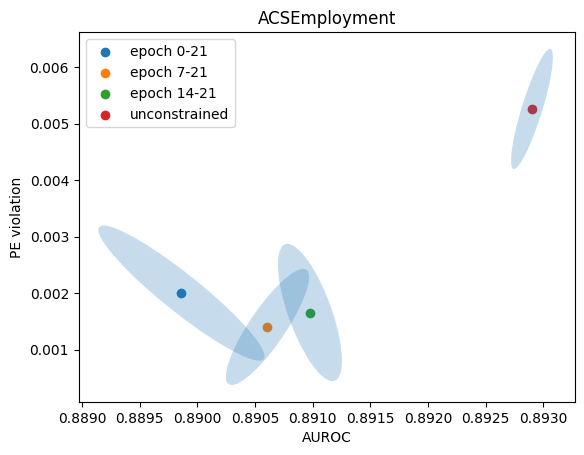
\includegraphics[width=0.45\textwidth]{assets/timing/ACSEmployment-PE.png}
    \hfill
    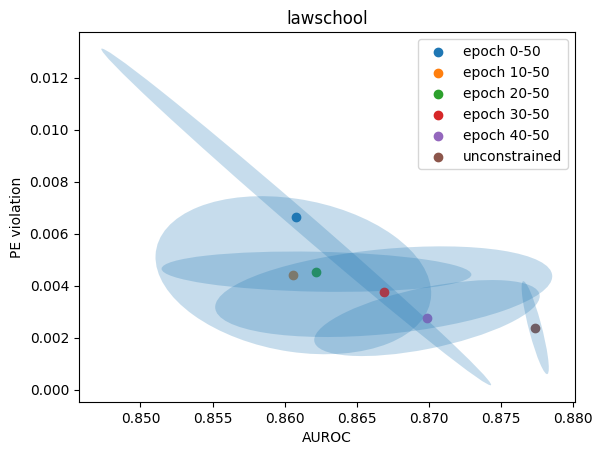
\includegraphics[width=0.45\textwidth]{assets/timing/lawschool-PE.png}
    \caption{PE perfomance plots using different ranges of fairness constrained training.}
\end{figure}
    
\begin{figure}[htbp]
    \centering
    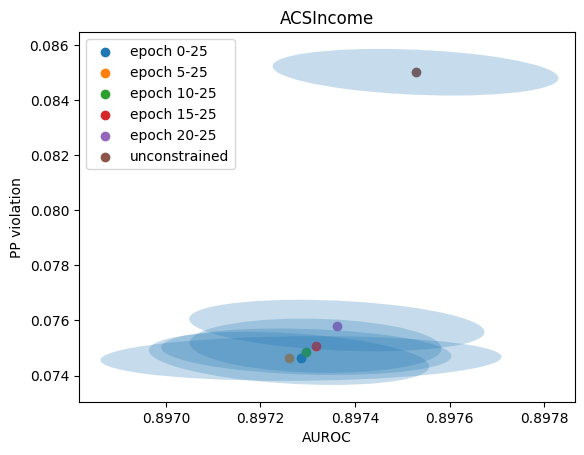
\includegraphics[width=0.45\textwidth]{assets/timing/ACSIncome-PP.png}
    \hfill
    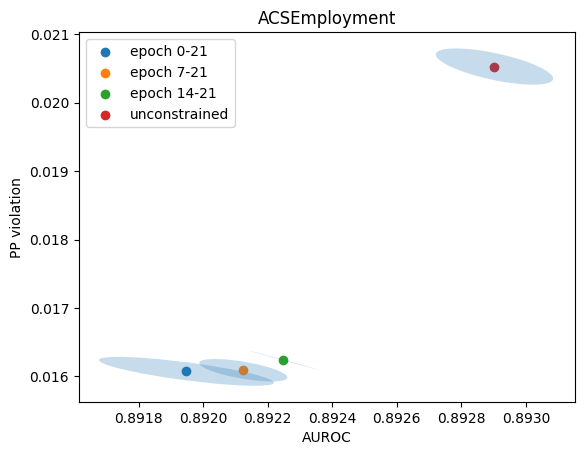
\includegraphics[width=0.45\textwidth]{assets/timing/ACSEmployment-PP.png}
    \hfill
    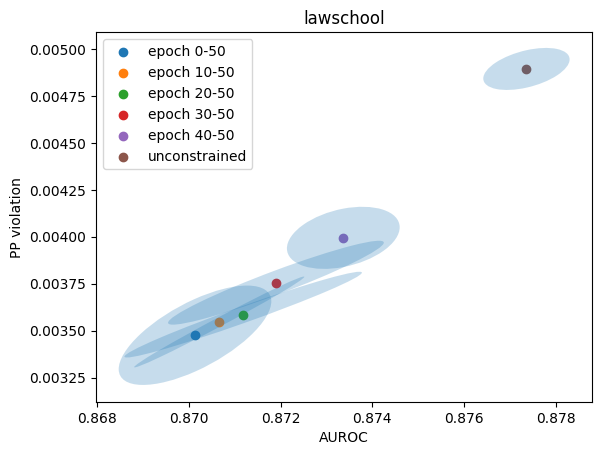
\includegraphics[width=0.45\textwidth]{assets/timing/lawschool-PP.png}
    \caption{PP perfomance plots using different ranges of fairness constrained training.}
\end{figure}
    
\begin{figure}[htbp]
    \centering
    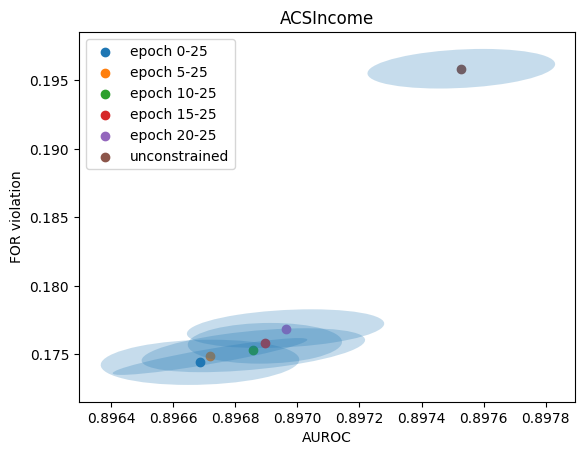
\includegraphics[width=0.45\textwidth]{assets/timing/ACSIncome-FOR.png}
    \hfill
    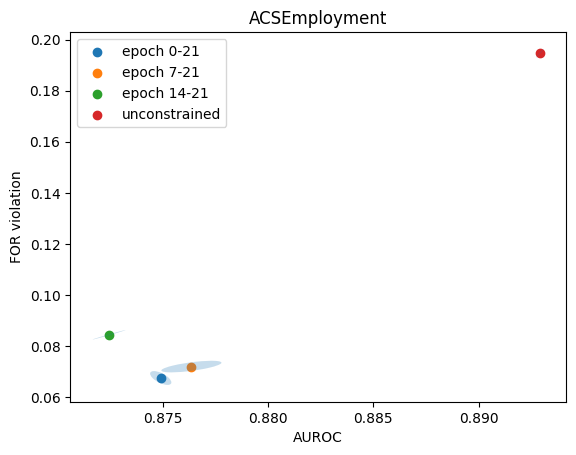
\includegraphics[width=0.45\textwidth]{assets/timing/ACSEmployment-FOR.png}
    \hfill
    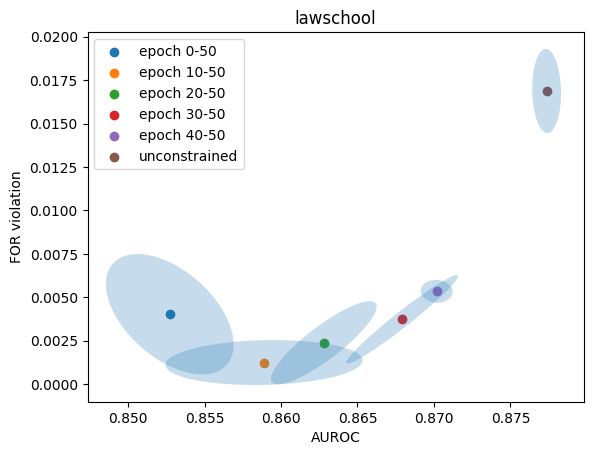
\includegraphics[width=0.45\textwidth]{assets/timing/lawschool-FOR.png}
    \caption{FOR perfomance plots using different ranges of fairness constrained training.}
\end{figure}
    
\begin{figure}[htbp]
    \centering
    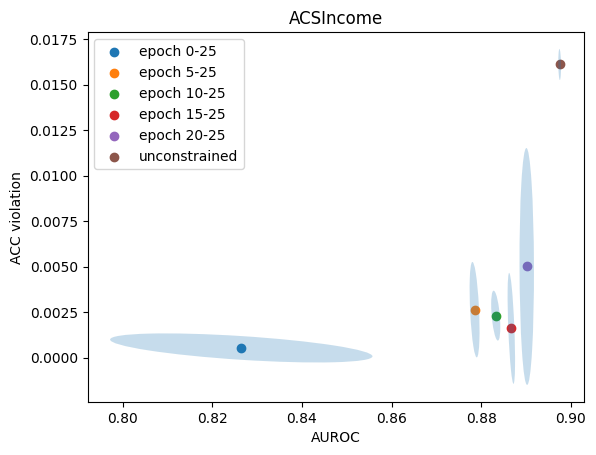
\includegraphics[width=0.45\textwidth]{assets/timing/ACSIncome-ACC.png}
    \hfill
    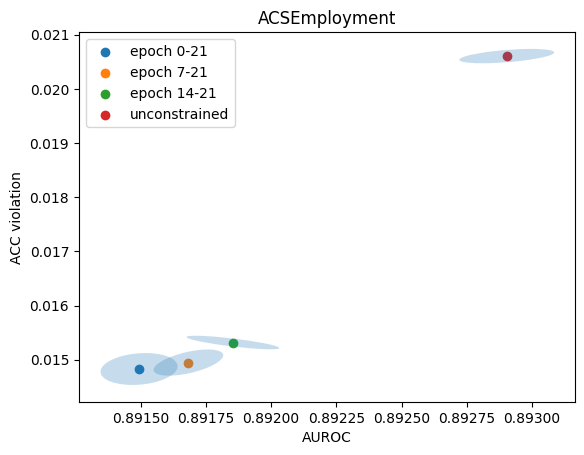
\includegraphics[width=0.45\textwidth]{assets/timing/ACSEmployment-ACC.png}
    \hfill
    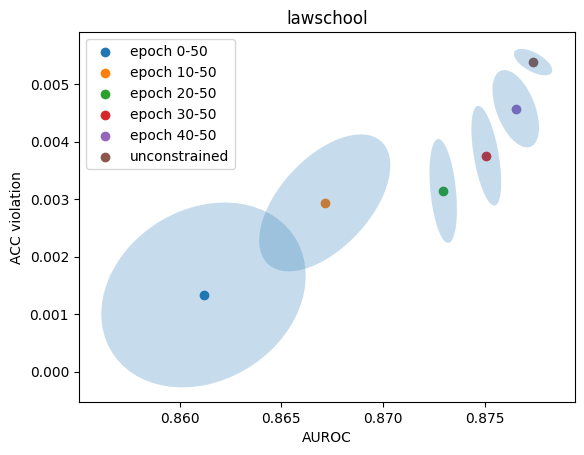
\includegraphics[width=0.45\textwidth]{assets/timing/lawschool-ACC.png}
    \caption{ACC perfomance plots using different ranges of fairness constrained training.}
    \label{fig:timingACC}
\end{figure}
    
\begin{figure}[htbp]
    \centering
    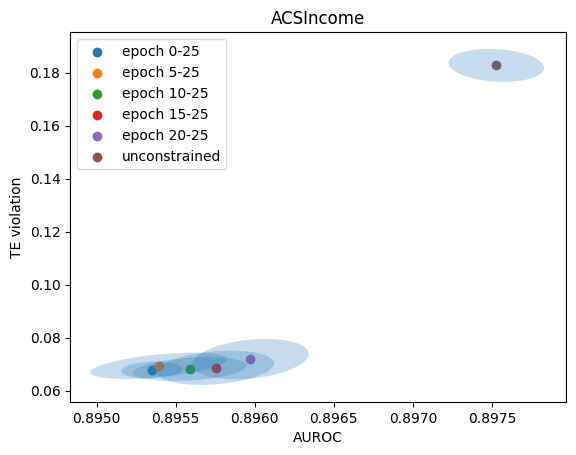
\includegraphics[width=0.45\textwidth]{assets/timing/ACSIncome-TE.png}
    \hfill
    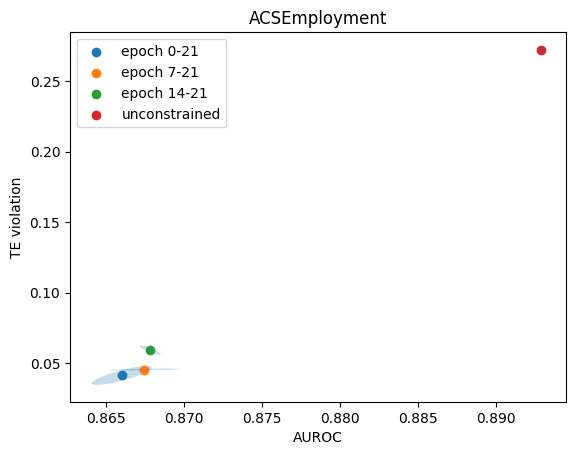
\includegraphics[width=0.45\textwidth]{assets/timing/ACSEmployment-TE.png}
    \hfill
    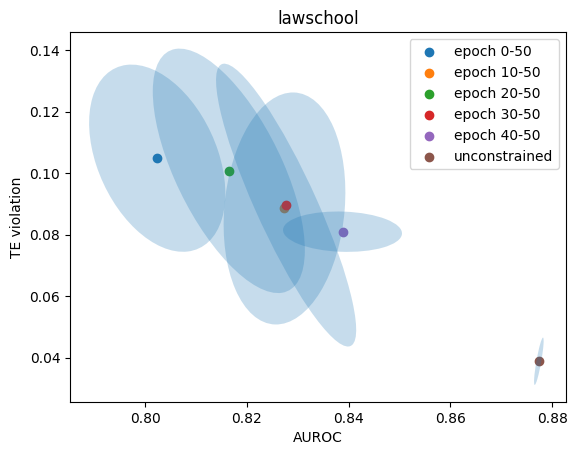
\includegraphics[width=0.45\textwidth]{assets/timing/lawschool-TE.png}
    \caption{TE perfomance plots using different ranges of fairness constrained training.}
    \label{fig:timingTE}
\end{figure}

\subsection{Training Dynamics}

The training dynamics for EO are shown in Figures~\ref{fig:timingEOval} and~\ref{fig:timingEOviol}. The violation curve shows that introducing the fairness constraint results in an immediate reduction in violation, after which there is little further improvement. The violation instead then becomes slightly unstable.

The performance curve shows a similar immediate effect when the constraint is introduced, with predictive performance decreasing at the first constrained training step. However, models that are branched earlier in training can continue to improve their performance after the constraint is introduced. For models branched later in training, performance continues to decrease after the constraint is applied, although the rate of this decrease becomes progressively smaller.

\begin{figure}[htbp]
    \centering
    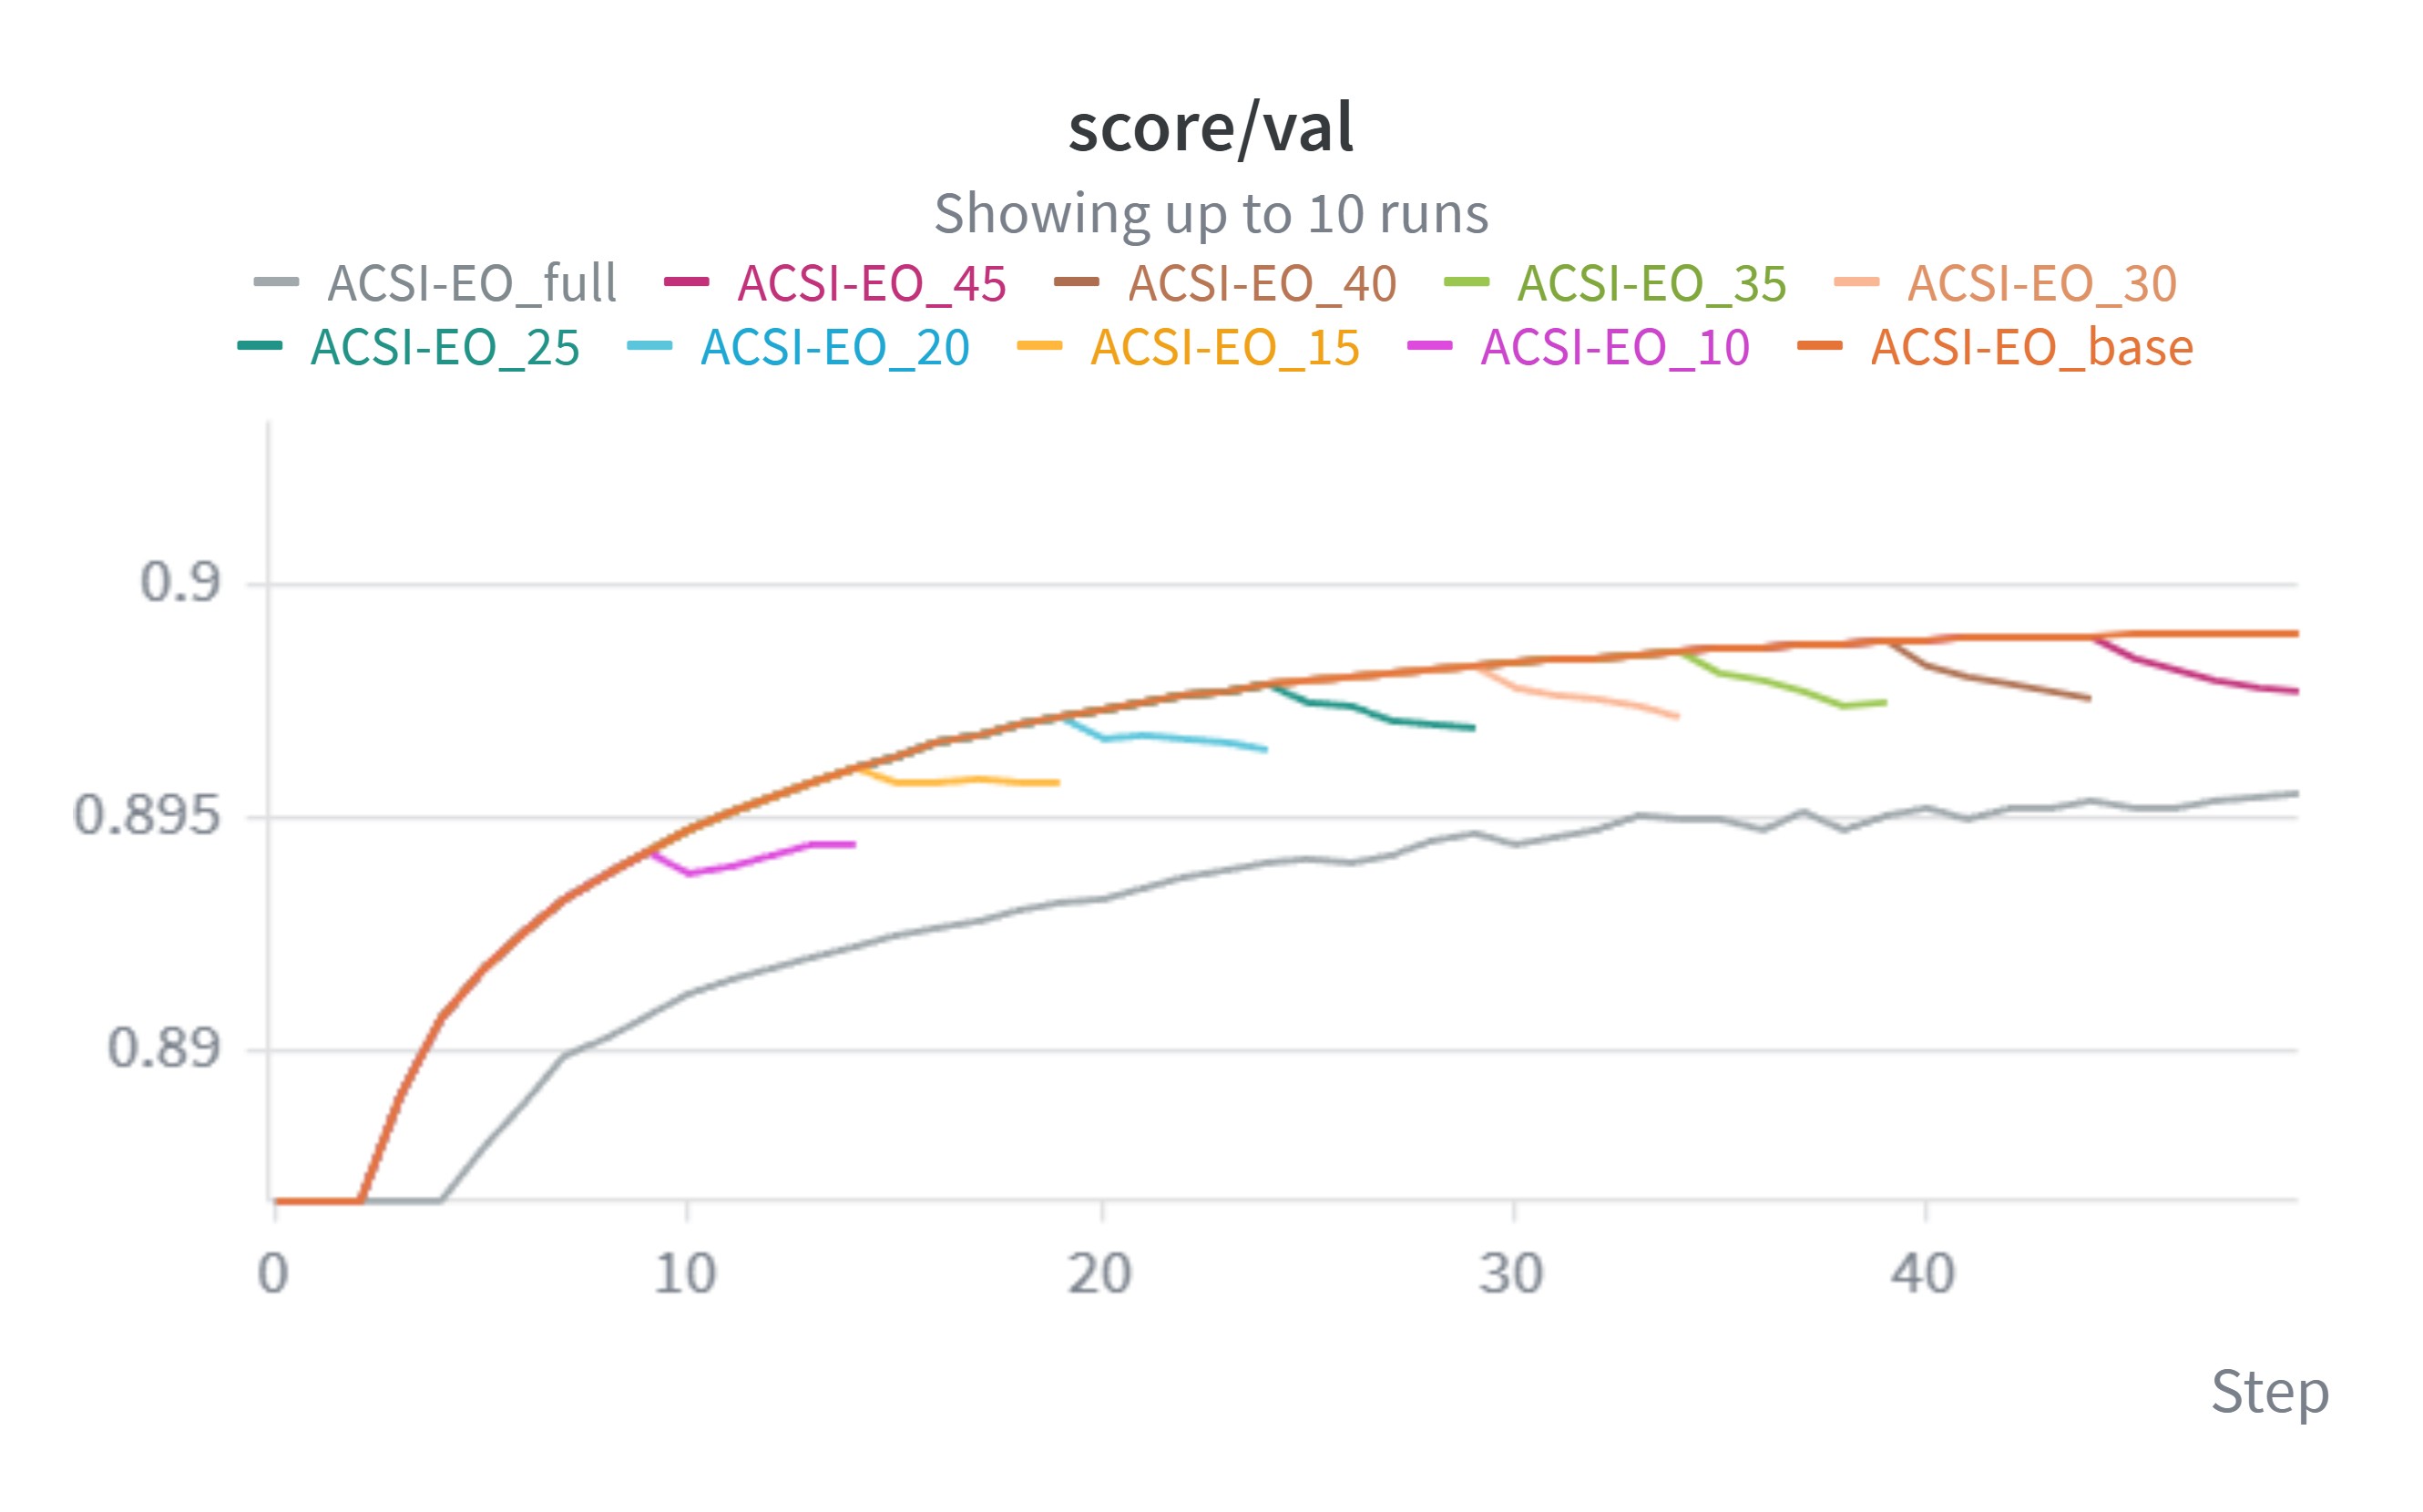
\includegraphics[width=0.9\textwidth]{assets/timing/startstop_score.png}
    \caption{Validation performance curves of an unconstrained model and a constrained model. At intervals of 5 epochs a model branches off the unconstrained model and is trained with constraints for 5 epochs.}
    \label{fig:timingEOval}
\end{figure}

\begin{figure}[htbp]
    \centering
    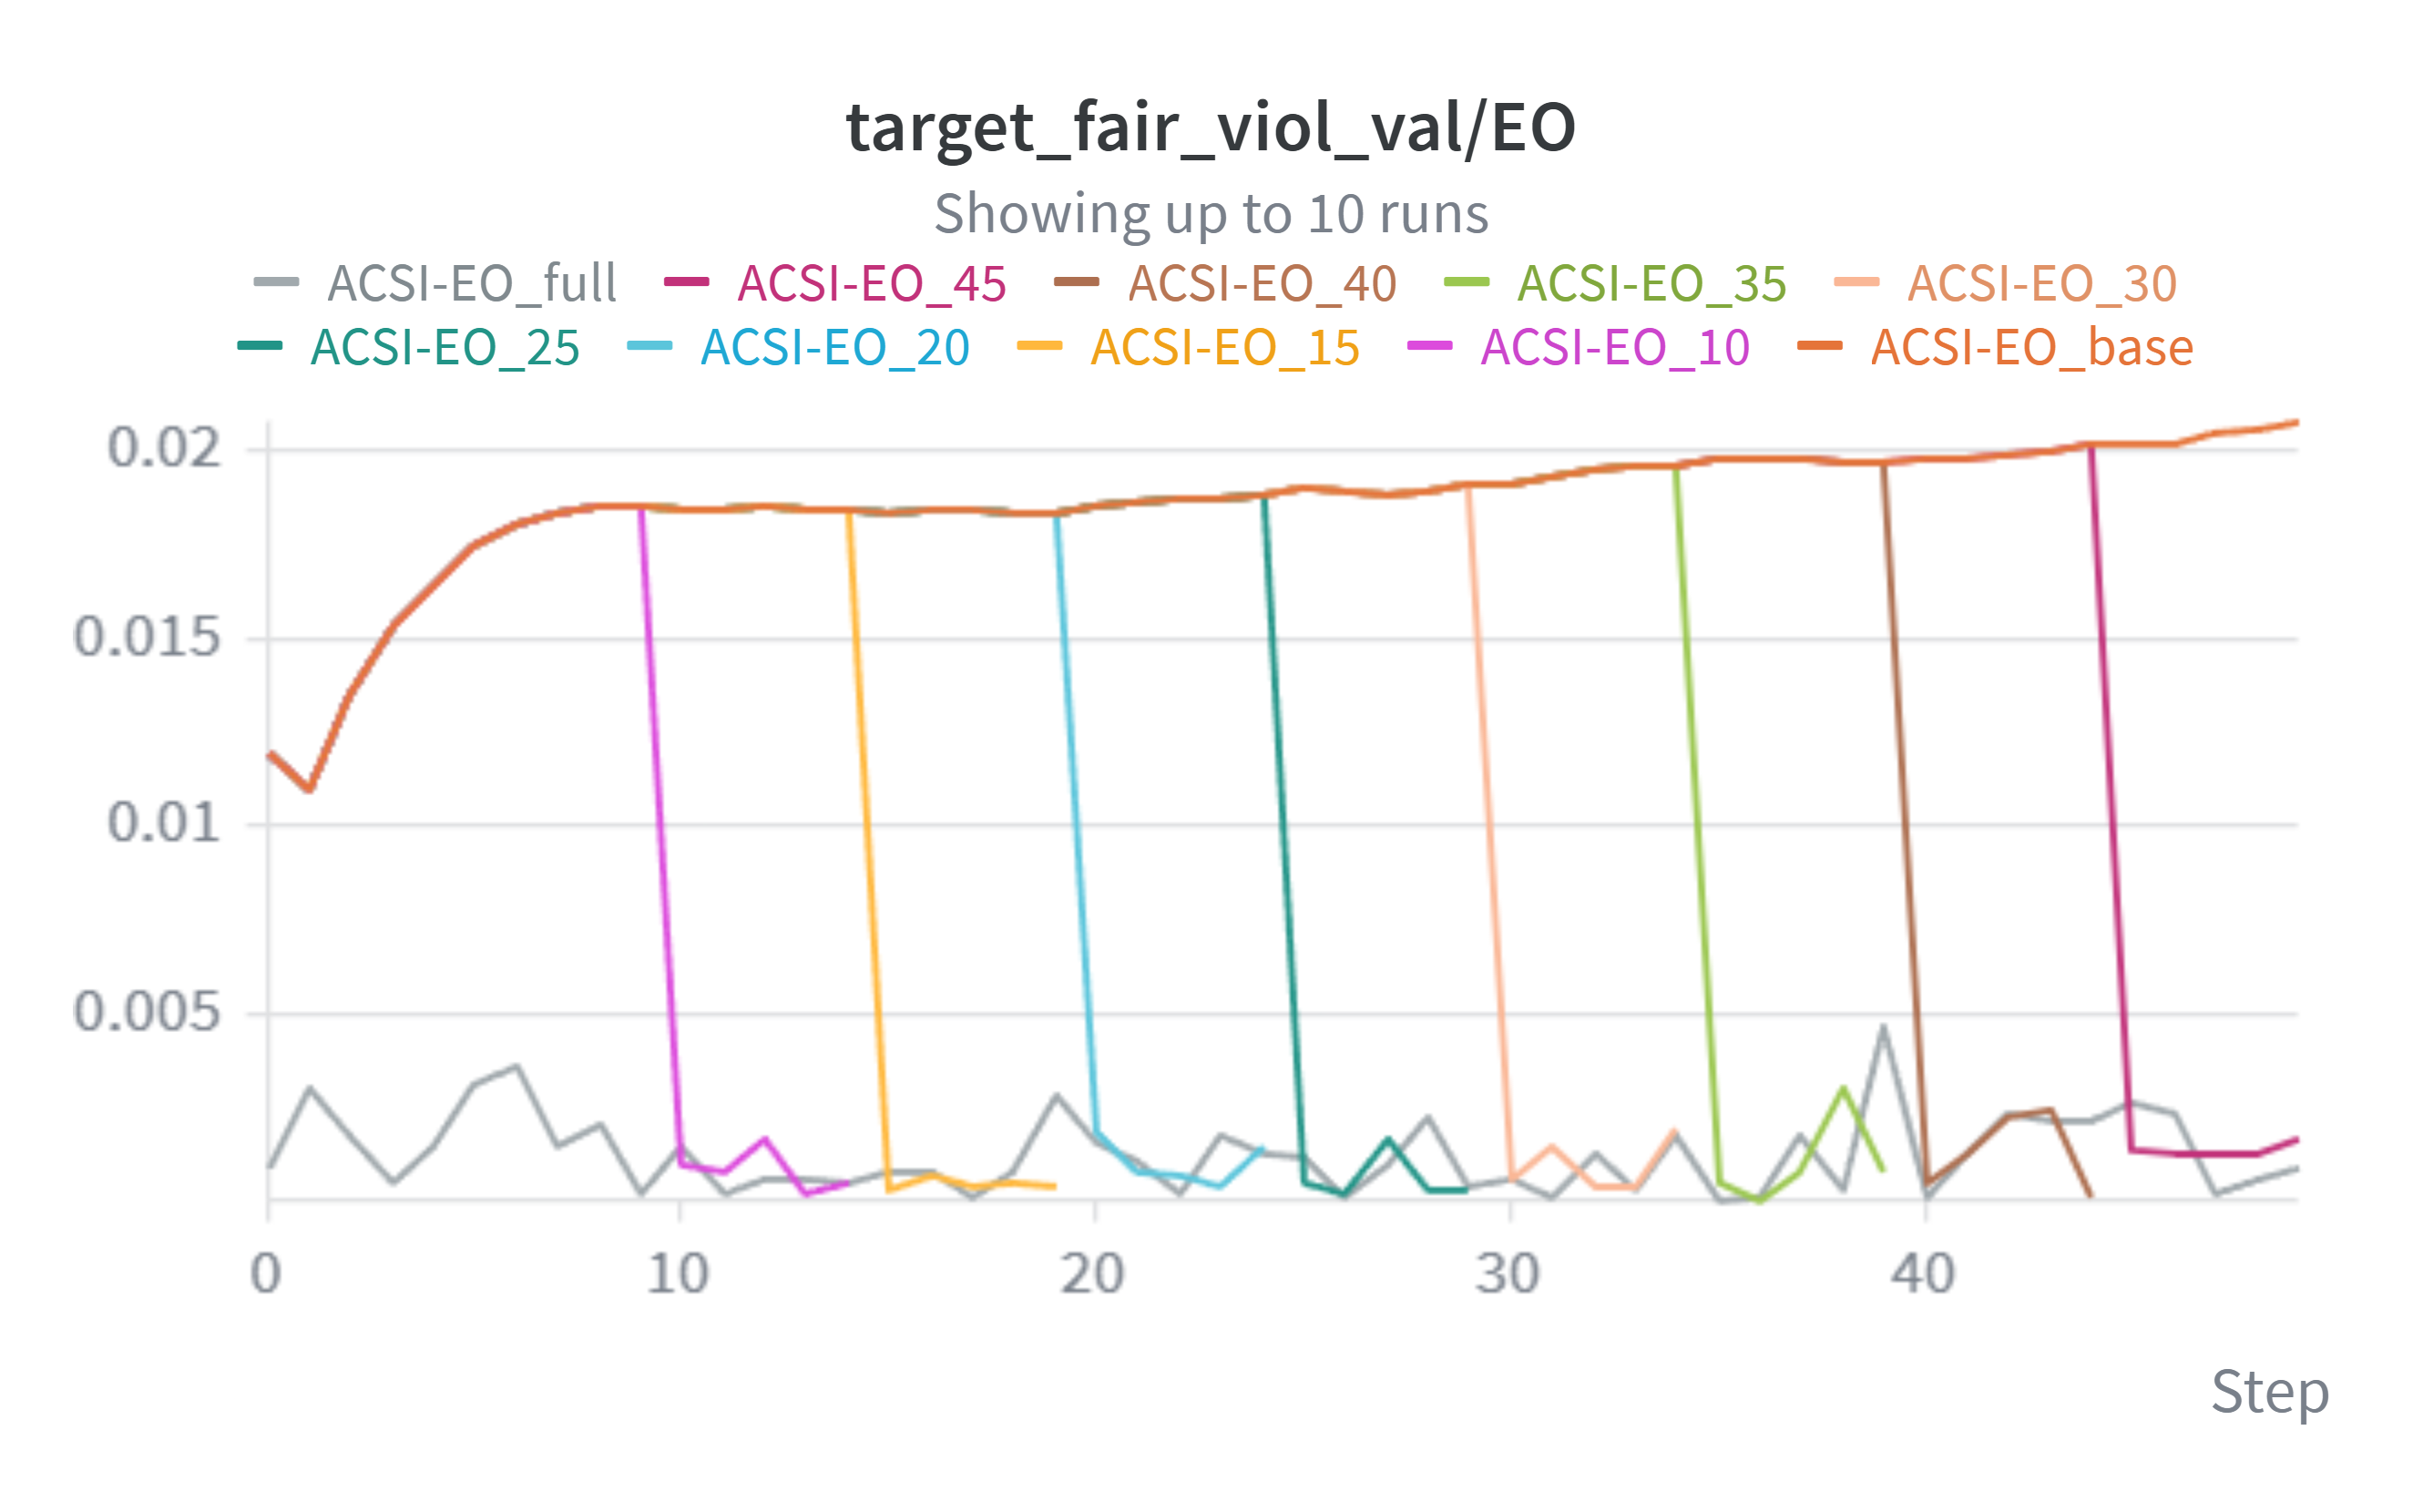
\includegraphics[width=0.9\textwidth]{assets/timing/startstop_eo.png}
    \caption{Validation EO violation curves of an unconstrained model and a constrained model. At intervals of 5 epochs another model branches off the unconstrained model and is trained with constraints for 5 epochs.}
    \label{fig:timingEOviol}
\end{figure}


\section{Discussion}
The purpose of this experiment was to determine whether fairness constraints need to be applied throughout training or whether they can be introduced later while still achieving comparable fairness using FAIRRETS. 

For all of the stable results, the fairness violation can be substantially reduced by applying the fairness constraint for only part of the training process. This indicates that the constraint does not necessarily need to influence the model throughout the entire training process to achieve a meaningful level of fairness. The training curves further support this, showing that much of the reduction in violation occurs shortly after the constraint is introduced.

The predictive performance decreases the longer a model was trained with a fairness constraint. However, this does not seem to be purely because of a performance-fairness trade-off in all cases. For the DP metric in Figure \ref{fig:timingDP}, when trained longer with a fairness constraint, the violation does not improve, yet the predictive performance gets worse. This is especially prevalent in the ACSIncome and lawschool datasets. Considering the unstable violation curve in Figure \ref{fig:timingEOviol}, this is likely because the constraint strength is too high as the model can no longer effectively decrease the violation rather than late constraint training improving performance.

Training an already capable, unconstrained model using a fairness constraint is perhaps the the favourable way of training a fair model with FAIRRETs. How this affects training behaviour is case by case depending on the configuration, dataset and metric used. The results show in some cases this method produces better results for both predictive performance and fairness. In other cases there is a performance-fairness trade-off. increasing the constraint can have the same effect rather than training longer. This is good news for FAIRRET, as this makes tuning a configuration for fairness can be done on a pre-trained, unconstrained model. This is significantly less computationally intensive than training a full model per configuration.